\documentclass{standalone}
\usepackage{tikz}
\usepackage{ctex,siunitx}
\usepackage{tkz-euclide}
\usepackage{amsmath}
\usetikzlibrary{patterns, calc}
\usetikzlibrary {decorations.pathmorphing, decorations.pathreplacing, decorations.shapes,}
\begin{document}
\small
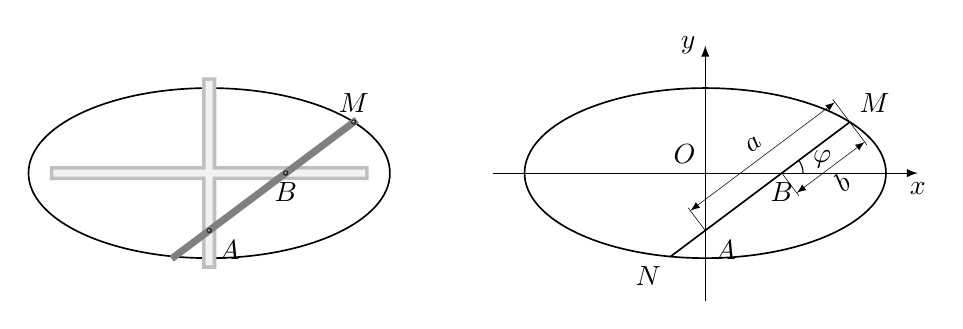
\begin{tikzpicture}[>=latex,scale=0.9]
  \begin{scope}
  \draw[thin,->](-3,0)--(3,0)node[below]{$x$};
  \draw[thin,->](0,-1.8)--(0,1.8)node[left]{$y$};
  \tkzDefPoints{0/0/O,0/-0.81/A,1.08/0/B,2.04/0.72/M,-0.4902/-1.1776/N,-0.24/-0.49/P,-0.21/-0.53/R,3/0/x}
  \tkzDefPointsBy[translation=from A to R](A,M){A',M'}
  \tkzDefPointsBy[translation=from R to A](B,M){B',M''}
  \tkzDefPointsBy[translation=from A to P](A,M){AP,MP}
  \tkzDefPointsBy[translation=from P to A](B,M){BP,MP'}
  \draw[very thin,<->](A')--(M')node[midway,sloped,above]{$a$};
  \draw[very thin,<->](B')--(M'')node[midway,sloped,below]{$b$};
  \tkzDrawSegments[very thin](A,AP M,MP B,BP M,MP')
  \draw[semithick](0,0)ellipse(2.55 and 1.2);
  \tkzMarkAngle[size=0.3](x,B,M)
  \tkzLabelAngle[pos=0.6](x,B,M){$\varphi$}
  \tkzDrawSegments[semithick](M,N)
  \tkzLabelPoints[above left](O)
  \tkzLabelPoints[above right](M)
  \tkzLabelPoints[below left](N)
  \tkzLabelPoints[below right](A)
  \tkzLabelPoints[below](B)
  \end{scope}
  \begin{scope}[xshift=-7cm]
    \draw[semithick](0,0)ellipse(2.55 and 1.2);
    \fill[lightgray] (-2.25,-0.1)rectangle(2.25,0.1)(-0.1,-1.35)rectangle(0.1,1.35);
    \fill[lightgray!20] (-2.2,-0.05)rectangle(2.2,0.05)(-0.05,-1.3)rectangle(0.05,1.3);
    \fill[gray] (-0.5,-1.2475)--(-0.56,-1.1675)--(2.05,0.79)--(2.11,0.71)--cycle;
    \fill[ball color=darkgray](0,-0.81)circle(1pt)node[below right]{$A$};
    \fill[ball color=darkgray](1.08,0)circle(1pt)node[below]{$B$};
    \fill[ball color=darkgray](2.04,0.72)circle(1pt)node[above]{$M$};
  \end{scope}
\end{tikzpicture}
\end{document}